\documentclass[10pt]{article}\usepackage[margin=.55in]{geometry}\usepackage[T1]{fontenc}\usepackage{graphicx}\setlength{\parindent}{0pt}\setlength{\parskip}{5pt}\sloppy\begin{document}{\large Exporter fixture compile failure preserved}\par Task T-1499. 3 November 2026.\par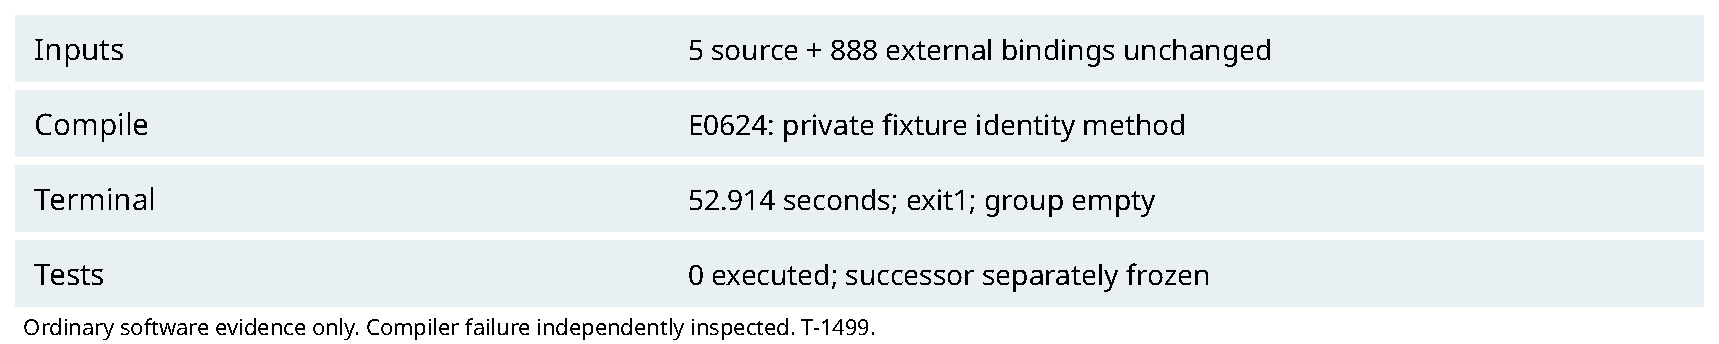
\includegraphics[width=\linewidth]{diagram.pdf}\par The bounded exporter compile reached an inaccessible fixture method: Spec::identity\_view is pub(crate), so the external test crate failed with E0624. No exporter or custody tests executed. The actual exporter and native validator implementations were unchanged.

The single authorized sequence lasted 52.914084 seconds, within its 120-second ceiling and hard 8 GiB address-space limit. Compiler and outer exit were 1. The compiler was reaped, its process group was empty, jobserver descriptors closed, and no pending signal or uncertain launch remained. All five source and 888 external input bindings matched before and after. No generated output remained.

Independent preflight review had identified two private fixture helpers and accepted their correction, but missed the remaining private spec identity method. The independent failed-attempt review records this miss. The predecessor coherent library build remains successful and is published separately; this receipt is not a test success.

A separate prospective successor constructs the exact four-field canonical identity object from public schema, workloads, arms and measurement fields, then calls public short\_id. It preserves all twelve assertions and native validators. That successor requires exact review and a distinct root release before execution.
\end{document}